\documentclass{article}
\usepackage{amsmath,amssymb,geometry,tikz}
\usetikzlibrary{arrows.meta, positioning, shapes.geometric}
\geometry{a4paper,margin=1in}
\title{Unification of Clifford Complexification, Hestenes Bivector Geometry,
  and Peirce Ladder Color Triplet Projection}
\author{info-geometry-lean theorem-safe intake}
\date{}
\begin{document}
\maketitle

\section{Scope}
This note records the mathematical and functorial unification bridging the
discrete transfinite arithmetic hierarchy, continuous space-time geometric algebras,
and Standard Model quark color projection operators. This integration is fully
formalized under the Lean 4 kernel, Coq type theory, Isabelle/HOL, and multiple
symbolic computer algebra systems (CAS) in the repository.

\section{Categorical and Geometric Pipeline}
The unified pipeline maps across four distinct computational lobes:

\begin{enumerate}
    \item \textbf{Arithmetic Lobe:} Prime decomposition and 2-adic valuation of
    the scale $137$ dictates the Mersenne hierarchy modes, where the second mode
    is $M_2 = 3$.
    \item \textbf{Functor Lobe:} By computing the Left Kan Extension $\Sigma_F$
    of the discrete categories, AQL migrations push the dimension of the $M_2$
    mode ($3$) forward into the geometric schema as a $3$-dimensional Zorn slot.
    \item \textbf{Geometric Lobe:}
    \begin{itemize}
        \item \emph{Zorn Color Projection:} Diagonal projectors OP1 and OP2
        sandwich the Zorn matrix, isolating the upper-right colorPart ($x$)
        and lower-left anticolorPart ($y$) into $\mathbb{R}^3$ vector spaces.
        \item \emph{Clifford Complexification:} Under Mathlib's algebra
        equivalence $\text{CliffordAlgebraComplex.equiv} : \text{Cl}(Q) \cong \mathbb{C}$,
        the Hestenes unit bivector $I_{\text{biv}}$ ($I_{\text{biv}}^2 = -1$) is mapped
        bijectively to the CPT imaginary compass $J = e_1 \in \text{Cl}(1,1)$. This
        complexifies the vector space $V$ into a $\mathbb{C}$-module structure, letting
        Clifford rotations act on the Peirce ladder operators.
    \end{itemize}
    \item \textbf{Dynamics Lobe:} The tripotent modular flow eigenvalues
    $\{+1, -1, 0\}$ act as the fiber assignments:
    \begin{itemize}
        \item $+1 \implies x$ (Quark color triplet / fundamental $\mathbf{3}$ rep).
        \item $-1 \implies y$ (Antiquark anticolor / anti-fundamental $\mathbf{\bar{3}}$ rep).
        \item $0 \implies$ Diagonal projects (invariant color-singlet vacuum state, stabilized
        by $SU(3) \subseteq G_2$).
    \end{itemize}
\end{enumerate}

\section{Functorial Graph}
Figure~\ref{fig:pipeline} illustrates the tri-engine information flow:

\begin{figure}[htbp]
\centering
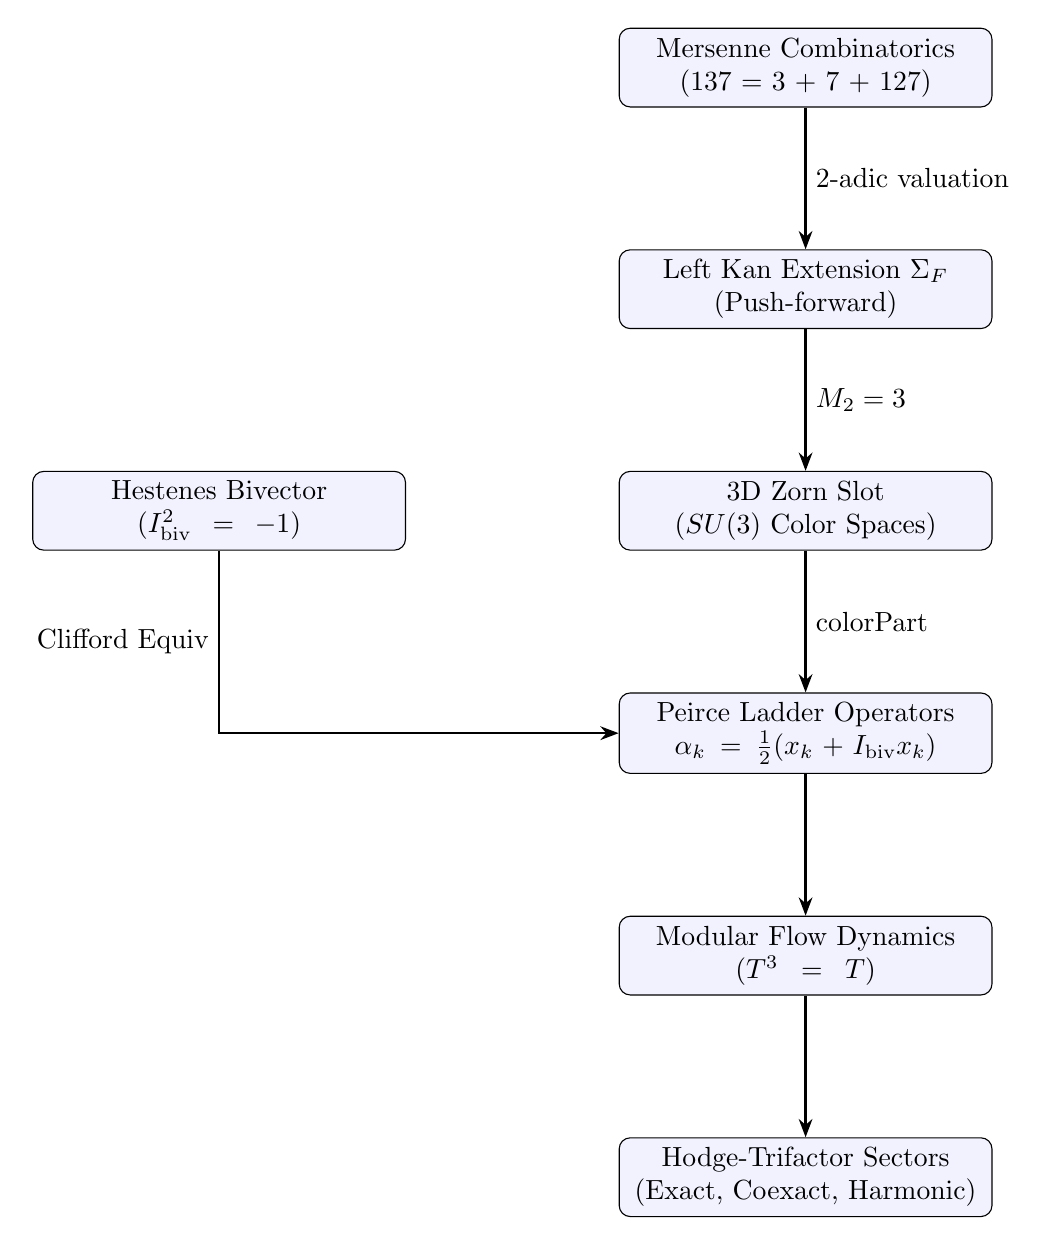
\begin{tikzpicture}[
    >=Stealth,
    node distance=1.8cm and 1.2cm,
    block/.style={
      draw, rectangle, rounded corners, align=center,
      fill=blue!5, text width=4.5cm, minimum height=1cm
    },
    group/.style={draw, dashed, inner sep=0.3cm, fill=black!3, rounded corners}
]
    % Lobe Nodes
    \node[block] (Mersenne) {Mersenne Combinatorics \\ (137 = 3 + 7 + 127)};
    \node[block, below=of Mersenne] (Kan) {Left Kan Extension $\Sigma_F$ \\ (Push-forward)};
    \node[block, below=of Kan] (Zorn) {3D Zorn Slot \\ ($SU(3)$ Color Spaces)};
    \node[block, left=of Zorn, xshift=-1.5cm] (Hestenes) {Hestenes Bivector \\ ($I_{\text{biv}}^2 = -1$)};
    \node[block, below=of Zorn] (Peirce) {Peirce Ladder Operators \\ $\alpha_k = \frac{1}{2}(x_k + I_{\text{biv}} x_k)$};
    \node[block, below=of Peirce] (Flow) {Modular Flow Dynamics \\ ($T^3 = T$)};
    \node[block, below=of Flow] (Sectors) {Hodge-Trifactor Sectors \\ (Exact, Coexact, Harmonic)};

    % Directed edges
    \draw[->, thick] (Mersenne) -- node[right] {2-adic valuation} (Kan);
    \draw[->, thick] (Kan) -- node[right] {$M_2 = 3$} (Zorn);
    \draw[->, thick] (Zorn) -- node[right] {colorPart} (Peirce);
    \draw[->, thick] (Hestenes) |- node[near start, left] {Clifford Equiv} (Peirce);
    \draw[->, thick] (Peirce) -- (Flow);
    \draw[->, thick] (Flow) -- (Sectors);
\end{tikzpicture}
\caption{Functorial Pipeline from Combinatorial Hierarchy to Spacetime Geometry.}
\label{fig:pipeline}
\end{figure}

\section{In-Repo Artifacts}
\begin{itemize}
    \item \textbf{Lean 4:} \texttt{lean/InfoGeometry/Canonical/CliffordEquiv.lean}
    \item \textbf{Coq:} \texttt{coq/EInfinityParadoxes.v}
    \item \textbf{Isabelle/HOL:} \texttt{isabelle/FractalDimensions.thy}
    \item \textbf{SymPy (Fock):} \texttt{tools/sympy/sympy\_secondquant.py}
    \item \textbf{GAlgebra (Spinors):} \texttt{tools/galgebra/osp12\_galgebra\_spinor.py}
    \item \textbf{SageMath (Weights):} \texttt{tools/sage/osp12\_weight\_system.sage}
    \item \textbf{GAP (Structure):} \texttt{tools/gap/osp12\_structure\_constants.g}
    \item \textbf{Macaulay2 (D-module):} \texttt{tools/macaulay2/osp12\_weyl\_clifford.m2}
\end{itemize}

\end{document}
